\begin{figure*}[t!]
   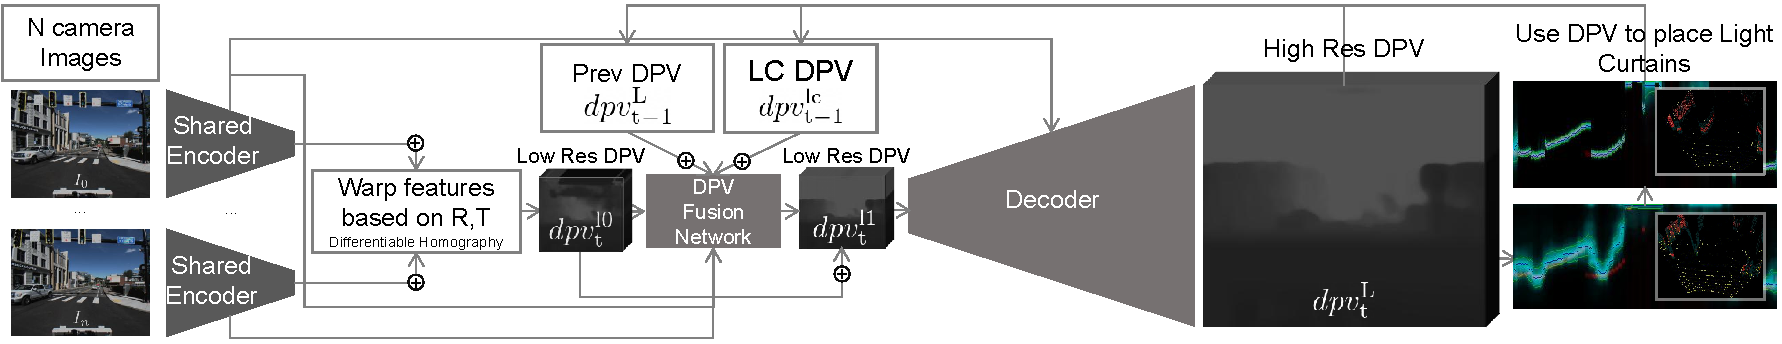
\includegraphics[width=1.0\textwidth]{figures/network.pdf}
   \caption{Our network takes in RGB images to generate a Depth Probability Volume (DPV). We then drive our Triangulation Light Curtain's laser to plan and place curtains on regions that are uncertain and refine it. This is then fed back on the next timestep to get much more refined DPV estimate.}
   \label{fig:network}
\end{figure*}
   
\section{Depth from Light Curtain + RGB Fusion}

\subsection{Motivation}

While starting from a uniform or gaussian prior with a large uncertainity is a valid option, it is slow to converge. Furthermore, a Light Curtain's only means of depth estimation is extracted primarily along the ruled placement of the curtain, at least based on our above placement policies. We would ideally like to use information from a Monocular RGB camera or Stereo Pair to initialize our prior, with a similar DPV representation. To this end, a Deep Learning based architecture is ideal, and we also reason that such an architecture could potentially learn to fuse/incorporate information from both modalities better.

\subsection{Structure of Network}

The first step is to build a network (Fig.~\ref{fig:network}) that can generate DPV's similar to our light curtain only estimation strategy from RGB images. To this end, we build upon the MVSNet/PSMNet \cite{chang2018pyramid} \cite{yao2018mvsnet} architecture. N images, usually 2 $I_{0}, I_{1}$ are fed into encoders that share weights, and the features are then warped into different fronto-parallel planes of the reference image $I_{0}$ using pre-computed $R_{i}^{0}, t_{i}^{0}$. Further convolutions are run to generate a low resolution DPV $dpv_{\mathrm{t}}^{\mathrm{l0}}$ [80, 96] where the log softmax operator is applied and regressed on. The transform between the camera's act as a constraint, forcing the feature maps to respect depth to channel correspondence. The add operator into a common feature map is similar to adding probabilities in log-space. 

This is then fed into the DPV Fusion Network (Set of 3D Convolutions) that incorporate a downsampled version of $dpv_{\mathrm{t-1}}^{\mathrm{L}}$ along with the the light curtain DPV that we had applied recursive bayesian updates on $dpv_{\mathrm{t-1}}^{\mathrm{lc}}$, and a residual is computed and added back to $dpv_{\mathrm{t}}^{\mathrm{l0}}$ to generate $dpv_{\mathrm{t}}^{\mathrm{l1}}$ to be regressed upon similarly. Occasionally, we train without this feedback by inputting a uniform distribution. Finally, this is then passed into a decoder with skip connections to generate a high resolution DPV $dpv_{\mathrm{t}}^{\mathrm{L}}$. This is then used to plan and place light curtains, from which we generate a new $dpv_{\mathrm{t}}^{\mathrm{lc}}$ to be fed in the next stage.

\subsection{Loss Functions}

\textbf{Soft Cross Entropy Loss:} We build upon the ideas found in \cite{Yang-2019-118007} and use a soft cross entropy loss function, with the ground truth lidar depthmap becoming a gaussian DPV with $\sigma_{gt}$ instead of a one hot vector. This way, when taking $\mathbb{E}\left(dpv^{gt}\right)$ we get the exact depth value instead of an approxmiation limited by the depth quantization $\D$. We also make the quantization slightly non-linear to have more steps between objects that are closer to the camera.
\small
\begin{align}
   l_{sce}=\frac{-\sum_{i}\sum_{d}\left(dpv^{\mathrm{\{l0,l1,L\}}}*log\left(dpv^{gt}\right)\right)}{n} \\
   \D=\{d_{0},\dots,d_{N-1}\};d_{q}=d_{\text{min}}+(d_{\text{max}}-d_{\text{min}})\cdot q^{pow}
  \label{eq:seloss}
\end{align}
\normalsize

\textbf{L/R Consistency Loss:} We train on both the Left and Right Images of the stereo pair where the Projection matrices $P_{l}, P_{r}$ are known \cite{godard2017unsupervised}. We enforce predicted Depth and RGB consistency by warping the Left Depthmap/Projected RGB into the Right Camera and vice-versa, and minimize the following metric:
\small
\begin{align}
   D_{l}=\mathbb{E}\left(dpv_{l}^{L}\right)\qquad D_{r}=\mathbb{E}\left(dpv_{r}^{L}\right) \\
   l_{dcl}=\frac{1}{n}\sum_{i}\left(\frac{\left|D_{\{l,r\}}-w\left(D_{\{r,l\}},P_{\{l,r\}}\right)\right|}{D_{\{l,r\}}+w\left(D_{\{r,l\}},P_{\{l,r\}}\right)}\right) \\
   l_{rcl}=\frac{1}{n}\sum_{i}\left(||I_{\{l,r\}}-w\left(I_{\{r,l\}},D_{\{l,r\}},P_{\{l,r\}}\right)||_{1}\right)
  \label{eq:lrcons} 
\end{align}
\normalsize

\textbf{Edge aware Smoothness Loss:} We ensure that neighbouring pixels have consistent surface normals, except on the edges/boundaries of objects with the Sobel operator $S_{x}, S_{y}$ via the term:
\small
\begin{align}
   l_{s}=\frac{1}{n}\sum_{i}\left(\left|\frac{\partial I}{\partial x}\right|e^{-|S_{x}I|}+\left|\frac{\partial I}{\partial y}\right|e^{-|S_{y}I|}\right)
  \label{eq:smooth} 
\end{align}
\normalsize

\subsection{Datasets}

We train and validate our algorithms on the KITTI dataset. We then trained the same network by initializing on those weights, but using our custom dataset to evaluate our algorithms on our sensor platform / jeep.

\begin{figure*}[h!]
  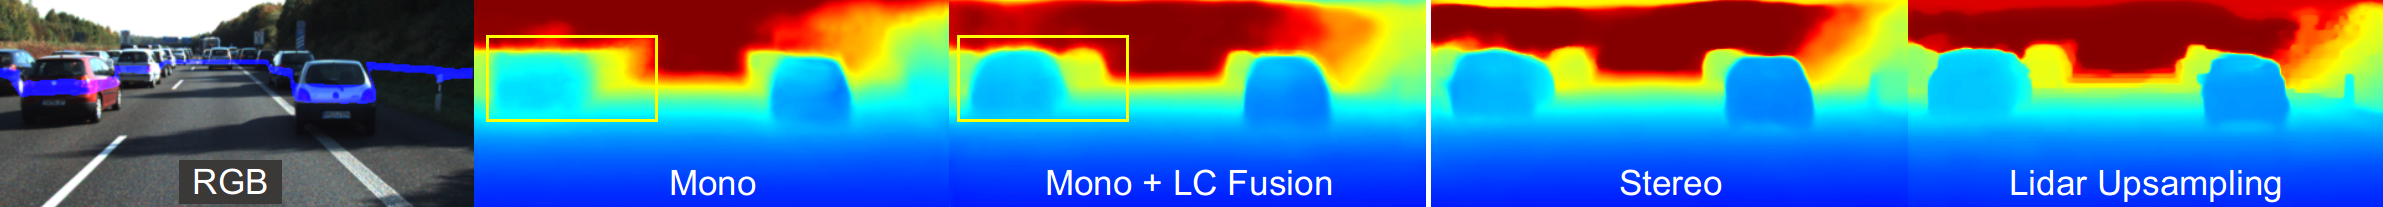
\includegraphics[width=1.0\textwidth]{figures/p1.png}
  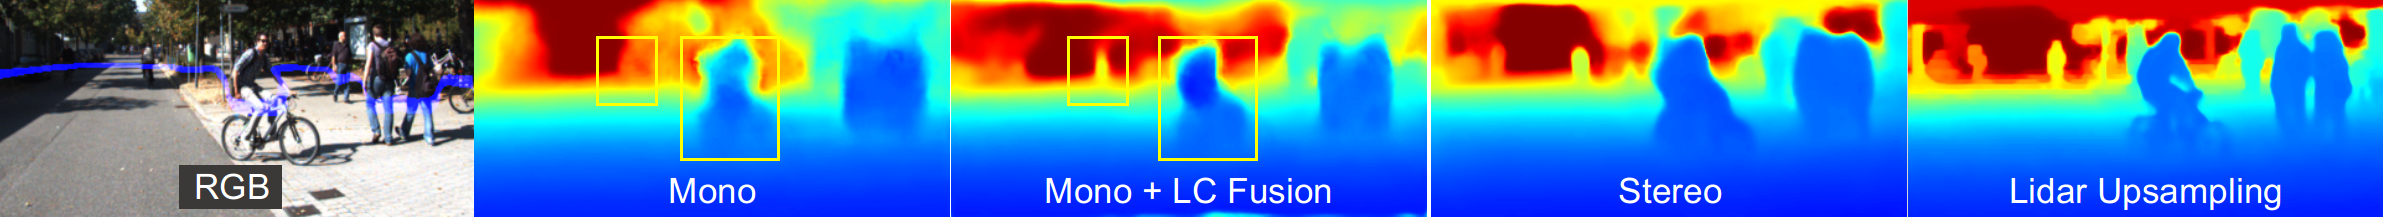
\includegraphics[width=1.0\textwidth]{figures/p2.png}
  \caption{In KITTI + Simulated Light Curtain, we note improved depthmaps when Monocular inputs are fused with Light Curtain inputs. Also, we note that the same architecture can be used Stereo Depth and Lidar Upsampling}  
  \label{fig:images2} 
\end{figure*}

\begin{figure*}[h!]
  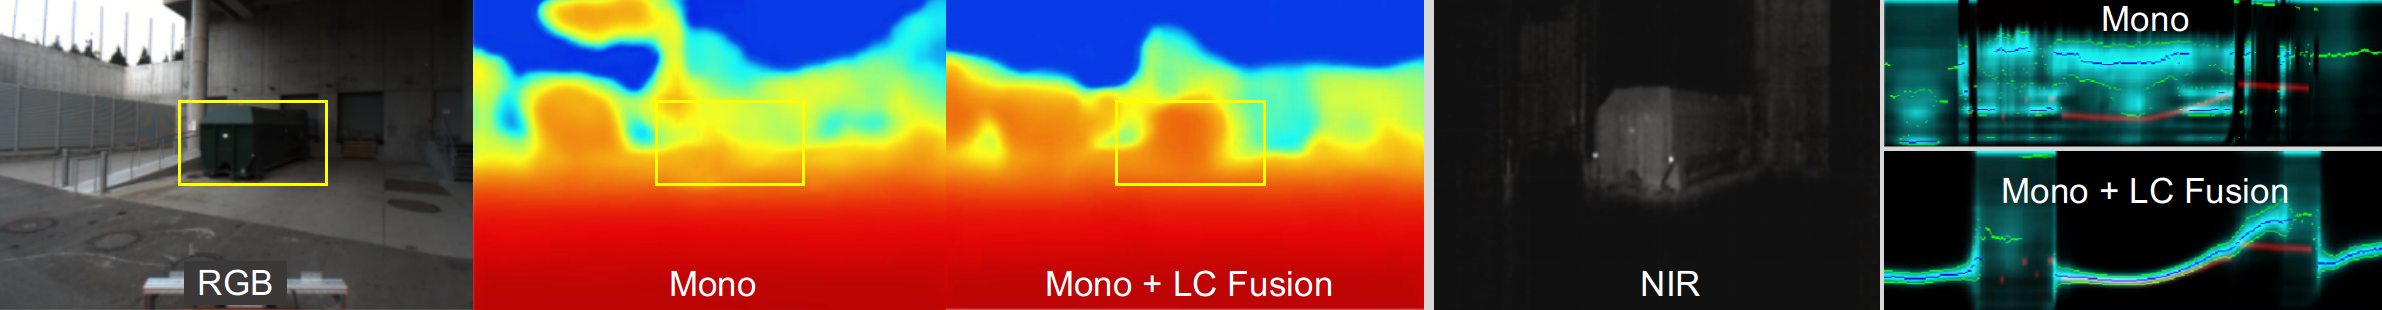
\includegraphics[width=1.0\textwidth]{figures/p4.png}
  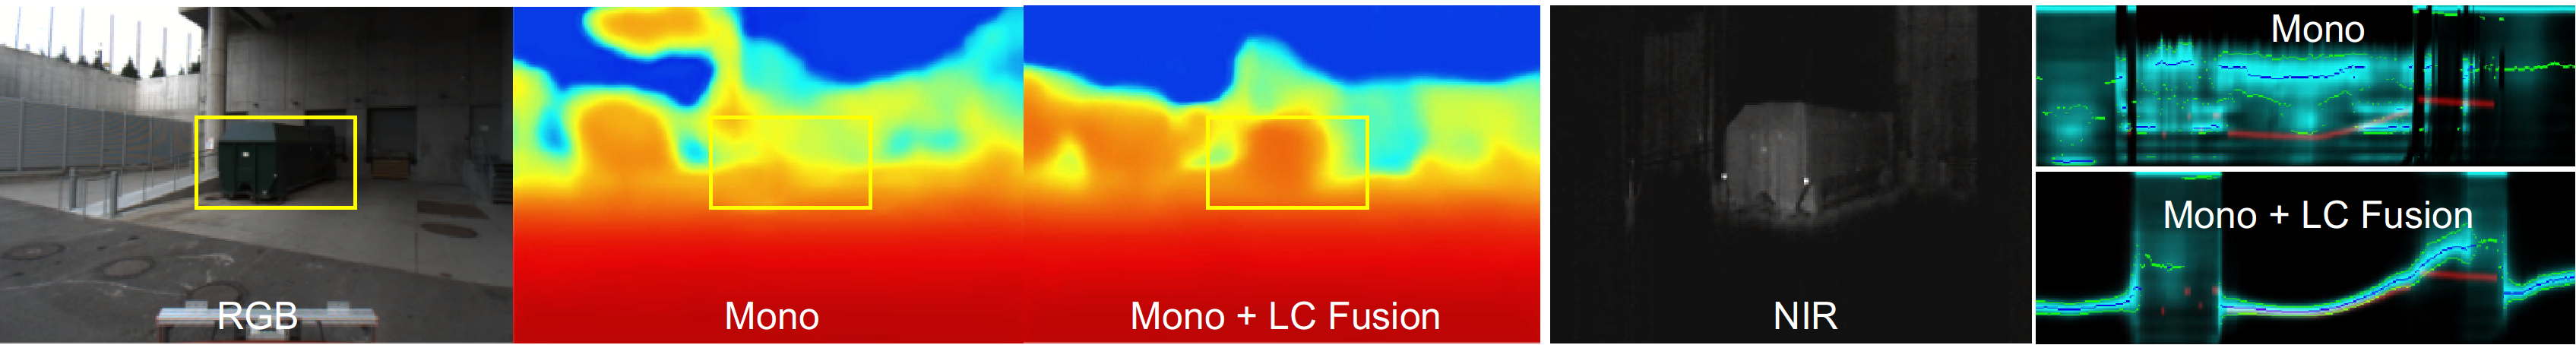
\includegraphics[width=1.0\textwidth]{figures/p5.png}
  \caption{In Real World Experiments, we are able to see the monocular scale ambiguity in domain specific scenarios get corrected by the Light Curtain, and we are able to see correction in any arbitary scene provided to the system as well}  
  \label{fig:images3} 
\end{figure*}

\begin{figure*}[h!]
  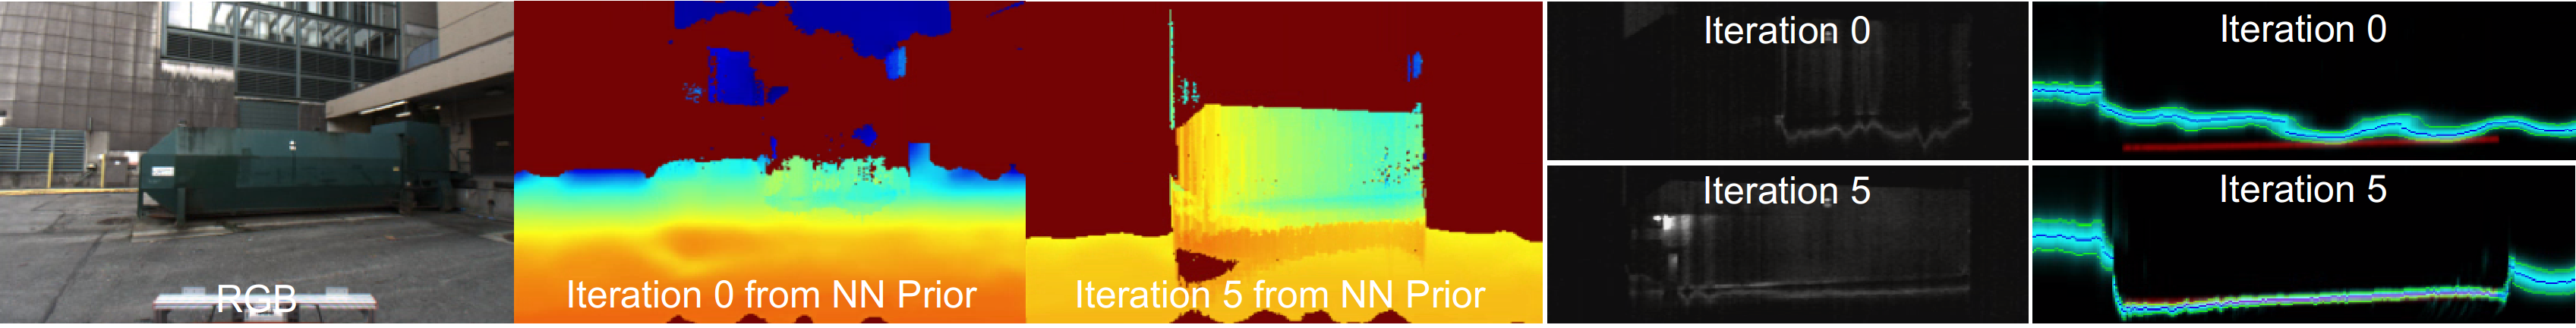
\includegraphics[width=1.0\textwidth]{figures/p6.png}
  \caption{We show the internal state of the bayesian update at Iteration 0 and Iteration 5. Starting with a prior DPV from Monocular Depth estimation, we show the convergence of the sensor's laser and curtain profile on an object 15m away}  
  \label{fig:images4} 
\end{figure*}

\begin{figure*}[h!]
   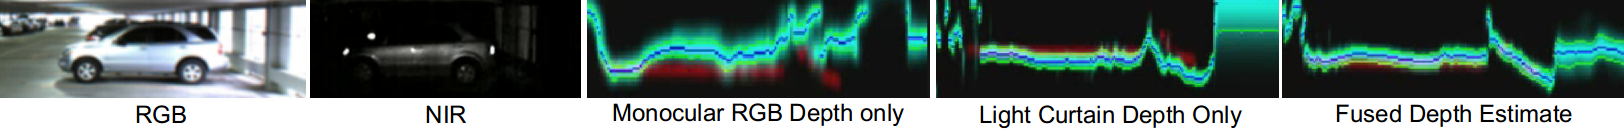
\includegraphics[width=1.0\textwidth]{figures/lastone4.png}
   \caption{Monocular RGB alone suffers from scale ambiguity but does give an inital uncertain depth estimate on a car 15m away. Iterating on Light Curtain measurements from a mean-centered gaussian prior alone gives a more accurate depth but with a noisy profile, but starting with the RGB DPV results in a more accurate and smoother profile.}  
   \label{fig:images5} 
 \end{figure*}

% \begin{figure}[h]
%    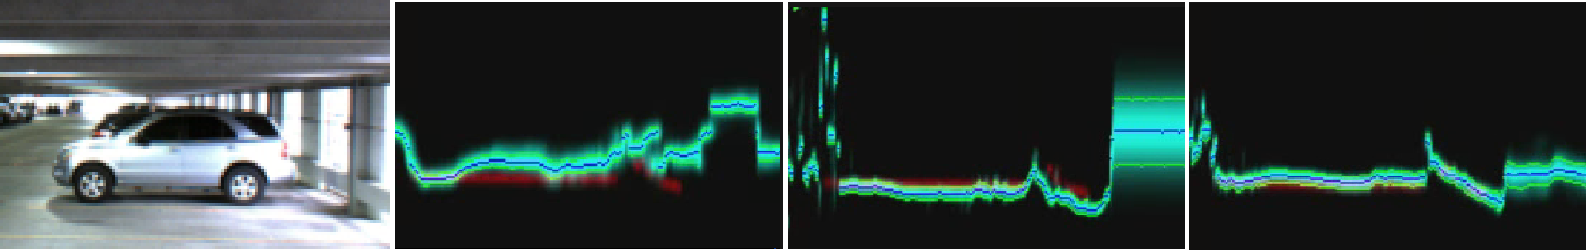
\includegraphics[width=0.46\textwidth]{figures/lastone.png}
%    \caption{We show the internal state of the bayesian update at Iteration 0 and Iteration 5}  
%    \label{fig:images5} 
%  \end{figure}

\section{Light Curtain + RGB Fusion Experiments} 

Here we consider the RMSE metric against the entire depthmap as opposed to just the Uncertainity Field (UF) as $\sqrt{\stackrel[i=1]{n}{\sum}\frac{\left(\mathbb{E}\left(\mathbf{d}_{u,v}\right)-\mathbf{d_{gt}}(u,v)_{i}\right)^{2}}{n}}$ against our ground truth.

\textbf{Effects of our loss function:} We do some simple experiments, training the task of monocular depth estimation, and we explore the effects of enabling various loss functions:
\noindent
\begin{table}[h]
  \centering
  \resizebox{0.5\linewidth}{!}{
  \begin{tabular}{|l|l|}
  \hline
   Parameters&  RMSE/m\\ \hline
   $\sigma_{gt}=0.05$ &3.24  \\ \hline
   $\sigma_{gt}=0.2$ &3.16  \\ \hline
   $\sigma_{gt}=0.3$ &3.06  \\ \hline
   $\sigma_{gt}=0.3$ with $l_{dcl}, l_{rcl}$  &2.93  \\ \hline
   $\sigma_{gt}=0.3$ with $l_{dcl}, l_{rcl}, l_{s}$  &2.90  \\ \hline
  \end{tabular}}
  \caption{Effects of Soft Cross Entropy ($\sigma_{gt}$), Left/Right Consistency ($l_{dcl}, l_{rcl}$), Smoothness losses ($l_{s}$) on Monocular Depth Estimation}
  \label{table:xx}
\end{table}

\vspace{-.1in}
We note succesively improving performance as we increase $\sigma_{gt}$, with poorer performance when the depth is effectively encoded as a one-hot vector (eg. $\sigma_{gt}=0.05$), since the depth was more likely to be forced into one of the categories in $\D$. Adding in $l_{dcl}, l_{rcl}$ and $l_{s}$ improved performance further, but we did not see any major performance improvement in varying $q^{pow}$ with $\sigma_{gt}$ was increased.

\textbf{Effect of Stereo Inputs:} We experiment with passing in a Monocular Pair at $t, t-1$, or a Stereo Pair at $t$, with $R,t$ known in both cases. We note significantly better performance with Stereo input. Note that our method can generalize to any N camera setup (Fig.~\ref{fig:stereodpv}).

\textbf{Effect of DPV Fusion Network:} We consider the task of Lidar Upsampling. The Velodyne Lidar in the KITTI dataset, can be converted into a low resolution depthmap, and consequently a low res DPV we call $dpv_{t}^{gt}$ . We could then fuse both $dpv_{t}^{l0}$ and $dpv_{t}^{gt}$ to generate $dpv_{t}^{l1}$ using Bayesian Inference. Alternatively, we could feed both of those inputs into our DPV Fusion Network above. We note improved performance in this upsampling task when using this approach as seen in Fig.~\ref{fig:stereodpv}. 

\begin{figure}[H]
  \centering
  \begin{minipage}{0.5\textwidth}
      \centering
      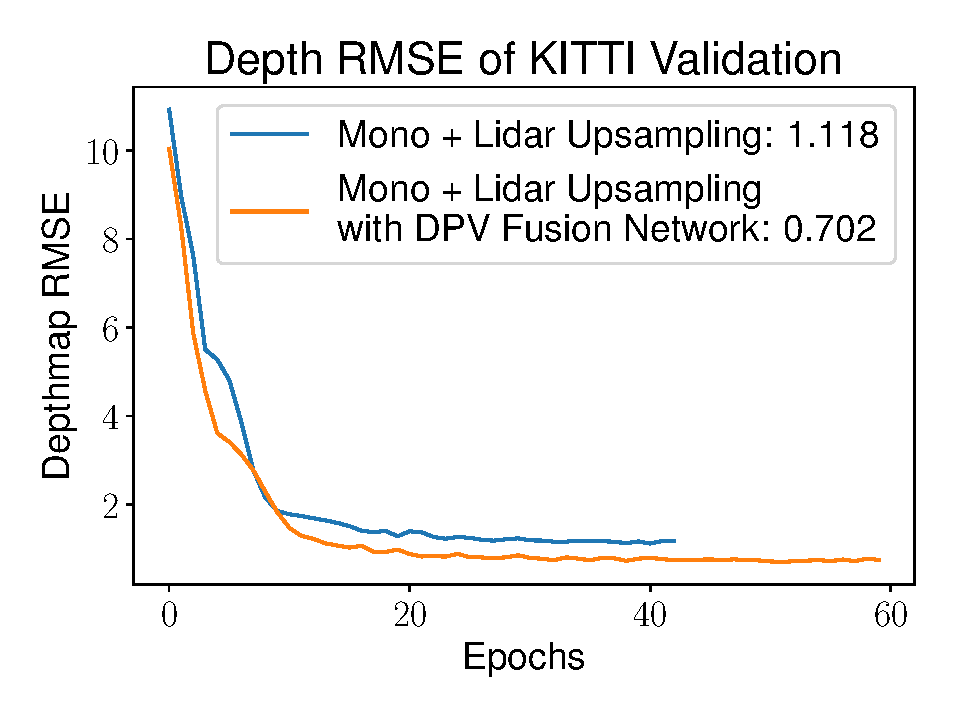
\includegraphics[width=0.49\textwidth]{figures/Figure_6.pdf}
      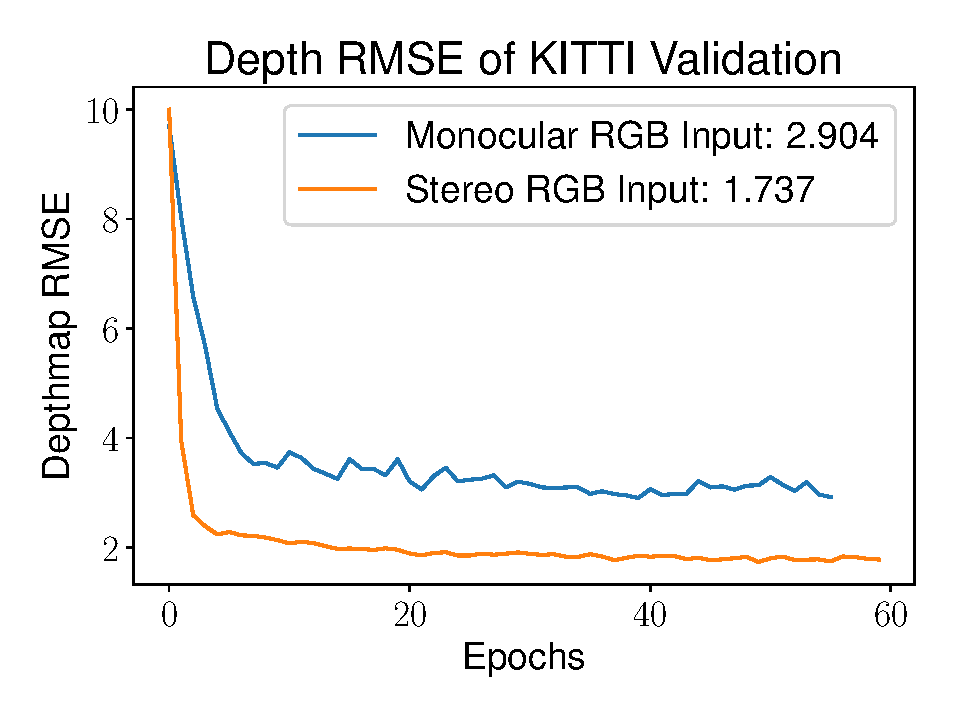
\includegraphics[width=0.49\textwidth]{figures/Figure_7.pdf}
  \end{minipage}\hfill
  \centering
  \caption{ \textbf{Left:} Same network but having a Stereo Pair at $t$ passed in instead of Monocular Pair at $t, t-1$. \textbf{Right:} Fusing the GT Lidar data with $dpv_{t}^{l0}$ to generate $dpv_{t}^{l1}$ and $dpv_{t}^{L}$ with Bayesian Inference vs DPV Fusion Network}
  \label{fig:stereodpv} 
\end{figure}

\textbf{Effect of a Stronger Prior:} Here, we show that a prior DPV generated from a monocular RGB camera as opposed to a mean-centered gaussian with a large $\sigma$ yields higher accuracy and faster convergence (Fig.~\ref{fig:images5}, Fig.~\ref{fig:prior}).

\begin{figure}[h]
  \centering
  \begin{minipage}{0.5\textwidth}
      \centering
      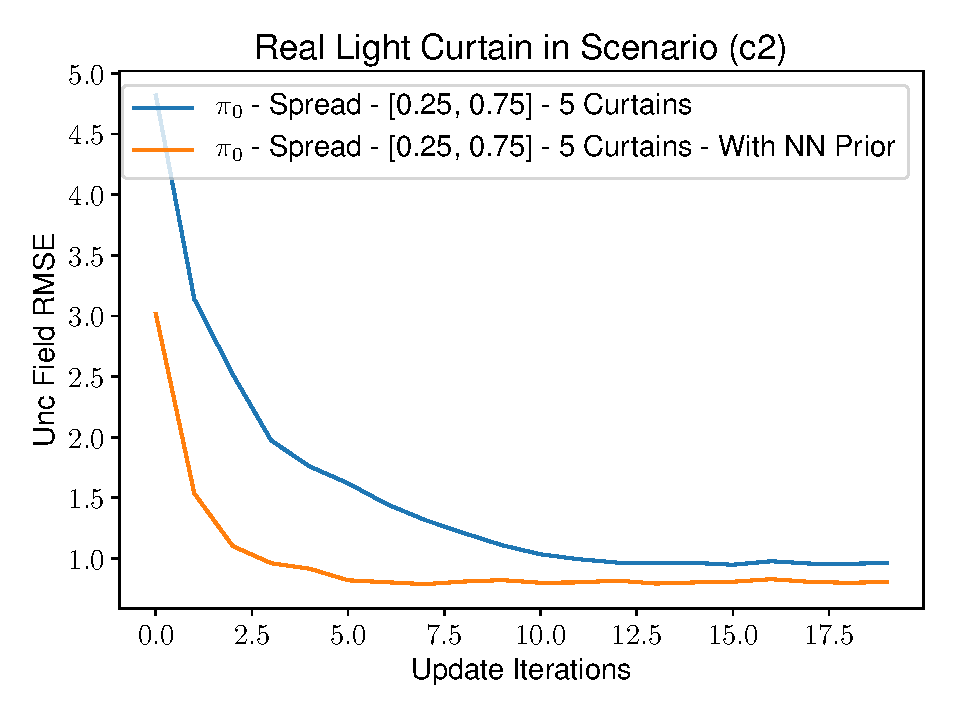
\includegraphics[width=0.49\textwidth]{figures/figure_X.pdf}
  \end{minipage}\hfill
  \centering
  \caption{Starting from a Prior distribution from a Monocular Depth Network as opposed to a mean-centered gaussian with a large $\sigma$ leads to faster discovery and convergence of true depth}
  \label{fig:prior} 
\end{figure}

\textbf{Effect of a Light Curtain Fusion:} Here, we train regular Monocular Depth Estimation without Light Curtain Feedback, and one where we enable $dpv_{t}^{lc}$ to be planned and fed-back on the next stage, on the KITTI dataset with our Light Curtain Simulator. We observed quantitative Fig.~\ref{fig:images3} and qualitative Fig.~\ref{fig:lfusion} performance improvement of depth with Monocular input, and minor improvement with Stereo.

\begin{figure}[h]
  \centering
  \begin{minipage}{0.5\textwidth}
      \centering
      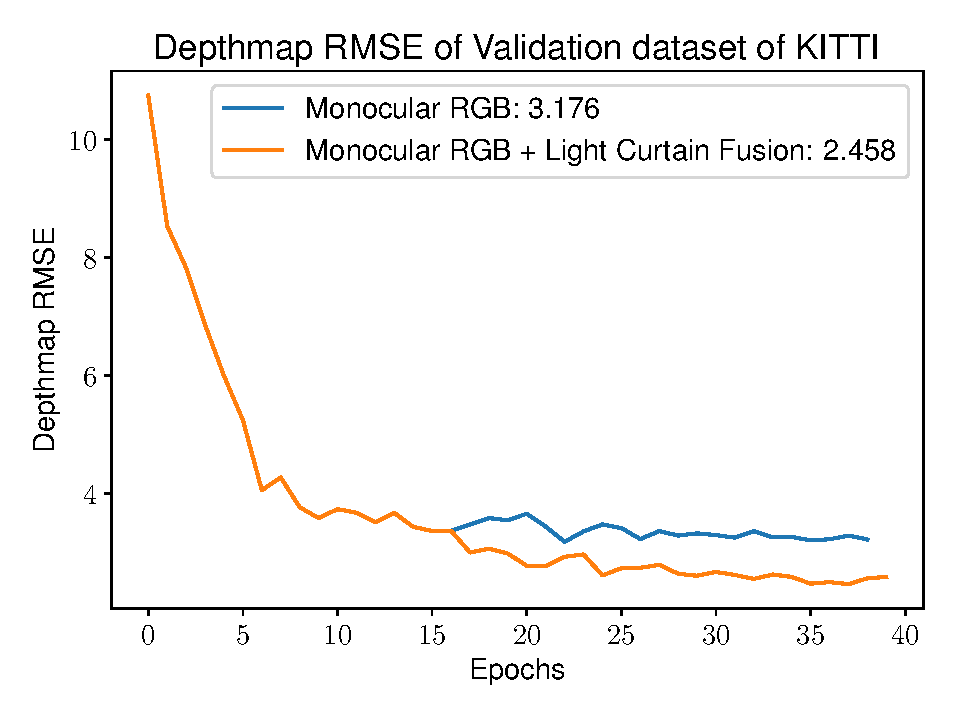
\includegraphics[width=0.49\textwidth]{figures/Figure_10.pdf}
      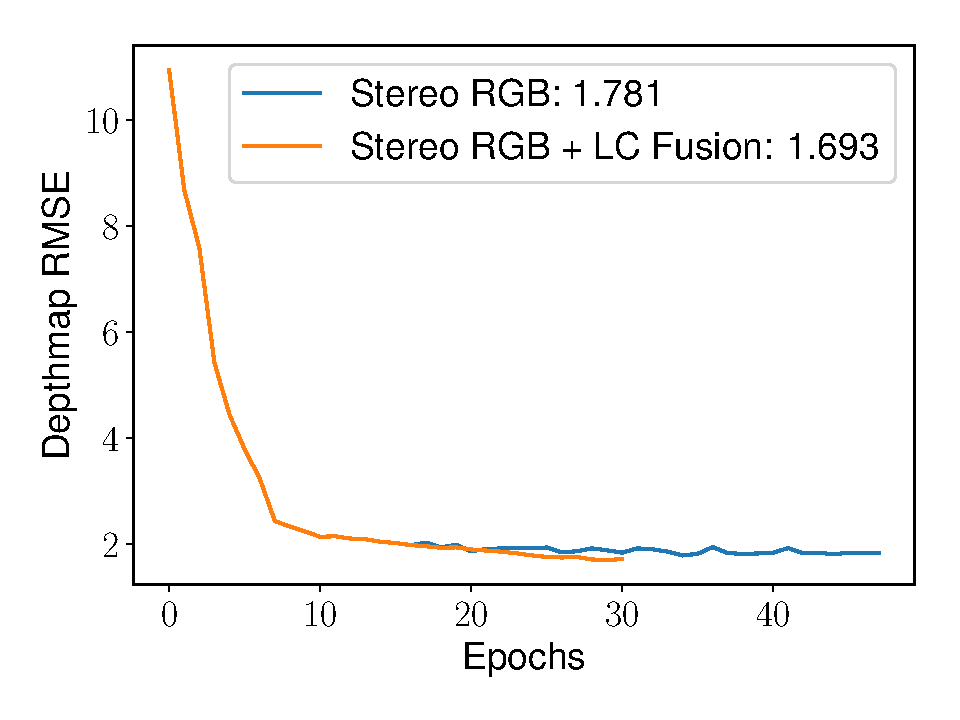
\includegraphics[width=0.49\textwidth]{figures/Figure_11.pdf}
  \end{minipage}\hfill
  \centering
  \caption{Monocular (Left) and Stereo (Right) Depth Estimation show improvement when we enabled feedback of the sensed Light Curtain DPV at epoch 16 when training on KITTI dataset with light curtain simulator}
  \label{fig:lfusion} 
\end{figure}

\subsection{Future Work}

We have demonstrated the first known work that has leveraged uncertainity in RGB cameras to drive an Adaptive Sensor such as a Light Curtain, in the context and large range operations of ADAS. Our approach \textit{can generalize} to any sensor that uses the principle of driving a laser or light source to specific pixels that are uncertain, and can benefit from depth uncertainity information of a pixel. 

Normally unincident and high reflectivity surfaces show poor intensity returns, so we hope to build a better sensor model that utilizes albedo and normal information. We could also extend this to temporaly inconsistent scenes (fast moving vehicle) by modelling scene flow.

\iffalse
Fig 15 maybe use the first image thing
Train Experiment on Fig 18 to show early LC feedback negative effect
Complete Future Work / Conclusion
\fi 






